%%%%%%%%%%%%%%%%%%%%%%%%%%%%%%%%%%%%%%%%%
% CU Boulder Physics Lab Writeup One Column
% LaTeX Template
% Version 1.0 (2022-10-05)
%
% This template has been downloaded from:
% http://www.LaTeXTemplates.com
%
% Original author:
% Mathias Legrand (legrand.mathias@gmail.com) titled Stylish Article 
% With extensive modifications by:
% Vel (vel@latextemplates.com)
% Further modifications for CU Boulder Physics by:
% Kristopher Bunker (kristopher.bunker@colorado.edu)
%
% License:
% CC BY-NC-SA 3.0 (http://creativecommons.org/licenses/by-nc-sa/3.0/)
%
%%%%%%%%%%%%%%%%%%%%%%%%%%%%%%%%%%%%%%%%%

%----------------------------------------------------------------------------------------
%	PACKAGES AND OTHER DOCUMENT CONFIGURATIONS
%----------------------------------------------------------------------------------------

\documentclass[10pt]{PhysLab1C} % Document font size

\usepackage[english]{babel} % Specify a different language here - english by default

%----------------------------------------------------------------------------------------
%	COLUMNS
%----------------------------------------------------------------------------------------

\setlength{\columnsep}{0.55cm} % Distance between the two columns of text
\setlength{\fboxrule}{0.75pt} % Width of the border around the abstract

%----------------------------------------------------------------------------------------
%	COLORS
%----------------------------------------------------------------------------------------

\definecolor{color1}{RGB}{0,0,90} % Color of the article title and sections
\definecolor{color2}{RGB}{0,20,20} % Color of the boxes behind the abstract and headings


%----------------------------------------------------------------------------------------
%	HYPERLINKS
%----------------------------------------------------------------------------------------

\usepackage{hyperref} % Required for hyperlinks

\hypersetup{
	hidelinks,
	colorlinks,
	breaklinks=true,
	urlcolor=color2,
	citecolor=color1,
	linkcolor=color1,
	bookmarksopen=false,
	pdftitle={Title},
	pdfauthor={Author},
}

%----------------------------------------------------------------------------------------
%	LAB AND COURSE INFORMATION
%----------------------------------------------------------------------------------------

\CourseInfo{Electronics for the Physical Sciences \vert ~ \textbf{PHYS 3330}} %
\Department{\copyright \ Department of Physics \vert ~ \textbf{University of Colorado Boulder} \ \vert ~ \textbf{\today}} %
\Copyright{\today} %
\LabTitle{Operational Amplifiers (OP-Amps) II} % Lab Title

%----------------------------------------------------------------------------------------
%	ABSTRACT
%----------------------------------------------------------------------------------------

\Abstract{\textbf{Lab 5:} Introduction to inverting amplifiers and other op-amp circuits.}

%----------------------------------------------------------------------------------------

\begin{document}

\maketitle % Output the title and abstract box

%\tableofcontents % Output the contents section

\thispagestyle{firstpage} % Removes page numbering from the first page

%----------------------------------------------------------------------------------------
%	ARTICLE CONTENTS
%----------------------------------------------------------------------------------------

\section{Goals}

In this lab, you will characterize the gain and frequency dependence of
inverting op-amp circuits. You will work with a few applications of
negative feedback including a circuit to sum voltages.

Proficiency with new equipment:

\begin{itemize}
\item
  Inverting op-amps: basic, summing, differentiator, and integrator
\end{itemize}

Experimental Design:

\begin{itemize}
\item
  Designing, building, and characterizing your own op-amp circuit
\end{itemize}

Modeling the physical system:

\begin{itemize}
\item
  Frequency dependence of op-amp circuits
\item
  Input and output impedances of op-amp circuits
\end{itemize}

Applications:

\begin{itemize}
\item
  Build a digital to analog converter
\end{itemize}

%------------------------------------------------

\section{Definitions}

\textbf{Closed-loop gain, $G$} - gain of the \emph{op-amp circuit} at all
frequencies with feedback applied

\textbf{Low frequency gain, $G_{0}$} - gain of the
\emph{op-amp circuit} at DC ($f$ = 0 Hz)

\textbf{Open-loop gain, $A$} - gain of the \emph{op-amp itself} at all
frequencies with no feedback applied

\textbf{DC gain, $A_{0}$} - gain of the \emph{op-amp itself}
at DC ($f$ = 0 Hz) with no feedback applied

\textbf{f\emph{\textsubscript{0}}} - 3 dB frequency for an \emph{op-amp
itself} with no feedback

\textbf{f\emph{\textsubscript{B}}} - 3 dB frequency for an \emph{op-amp
circuit} with feedback applied

\textbf{f\emph{\textsubscript{T }}}- unity gain frequency, frequency
where the open loop gain A is equal to one

%------------------------------------------------

\section{Inverting Amplifier Theory}

\begin{figure}[h]
 \centering
 \begin{circuitikz}[american voltages]
    \draw (0,0) node[op amp, anchor=-](OA){\texttt{}} 
    (OA.+) -- ++((-.5,0) to ++(0,-.5) node[ground]{}
    (OA.-) -- ++((-.5,0) to ++(0,1) coordinate(FC) to [R, l_=$R$, *-] ++(-2,0)
    to [short, -o] ++(0,0) node[anchor = east]{$V_{in}$}
    (FC) -- ++(.75,0) to [R=$R_F$] ++(1.5,0) to [short] ++(1,0) coordinate(FD)
    (FD) to [short, -*] (OA.out -| FD){}
    (OA.out) to [short, -o] ++(1.5,0) node[anchor = west]{$V_{out}$}
    ;
 \end{circuitikz}
 \caption{Inverting amplifier}
  \label{invamp}
\end{figure}


The basic inverting amplifier is shown in Figure \ref{invamp}. We can use the
Golden Rules to determine the low-frequency gain. Since the positive
input is grounded, the op-amp will do everything it can to keep the
negative input at ground as well. In the limit of infinite open loop
gain the inverting input of the op-amp is a \underline{virtual ground}, a
circuit node that will stay at ground as long as the circuit is working,
even though it is not directly connected to ground. When \emph{\textbf{A
is infinite,}} the gain of an inverting amplifier is

\[G_0=\frac{V_{out}}{V_{in}}=-\frac{R_f}{R}\]

This is the "Golden Rule" result. For the frequency dependence of the
gain we need to consider what happens when $A$ is not infinite, as we did
for the non-inverting case. We use the same definitions as for the
non-inverting case. The op-amp open loop gain is $A$, and the divider
ratio $B$ is the same as before:

\[B=\frac{R}{R+R_f}\]

When \emph{\textbf{A is finite}} the gain for an inverting amplifier is
given by

\[G_0=\frac{V_{out}}{V_{in}}=-\frac{A(1-B)}{1+AB}\]

The above formulas are still correct when \(A\) and/or \(B\) depend on
frequency. \(B\) will be frequency independent if we only have resistors
(in other cases that use complex impedance it may not be), but \(A\)
always varies with frequency. For most op-amps, including the LF356, the
open loop gain varies with frequency like an RC low-pass filter:

\[A(f)=\frac{A_0}{1+j\frac{f}{f_0}}\]

The 3 B frequency, \(f_0\), is usually very low, around 10 Hz. Data
sheets do not usually give \(f_0\) directly; instead they give the DC
gain, $A_0$, and the unity gain frequency \(f_T\), which is the frequency
where the magnitude of the open loop gain \(A\) is equal to one. The
relation between \(A_0\), \(f_0\), and $f\_T$ is

\[f_{T} = A_{0}f_{0}\]

The frequency dependence of the closed loop gain $G$ is then given by

\[G=\frac{G_0}{1+j\frac{f}{f_B}}\]

The frequency response of the amplifier with feedback is therefore also
the same as for an RC low-pass filter.

\subsection{Input and output impedances of inverting amplifiers}

Formulas for the input and output impedance for an inverting amplifier
are derived in H\&H Section 4.26. When the open loop gain is large, the
negative input of the op-amp is a virtual ground and so the input
impedance is just equal to $R$. This is very different from the
non-inverting case where the input impedance is proportional to $A$ for
large $A$. In practice, the input impedance of an inverting amplifier is
not usually greater than about 100 k$\Omega$, while the input impedance of a
non-inverting amplifier can easily be as large as 10\textsuperscript{12}
$\Omega$. When $A$ is not large the formulas for the input impedance and output
impedance of the entire circuit are derived in H\&H Section 4.26. The
results are

\[R_{i}^{'} = R + \frac{R_{f}}{1 + A}\]

\[R_{o}^{'} = \frac{R_{o}}{(1 + AB)}\]

The output impedance is the same for both the inverting and
non-inverting amplifiers.

The gain-bandwidth product for inverting amplifier is slightly modified
compared to non-inverting amps.

\[A_{0}f_{0} = \frac{{{- G}_{0}f}_{B}}{1 - B} = f_{T}\]

This is the same (except for the sign) as the non-inverting result when
the closed loop gain is large (\(B \ll 1, |G0| \gg 1\)), but at unity
closed loop gain (\(B = 1/2, G_0 = -1\)) the inverting amplifier has
only half as much bandwidth as a non-inverting amplifier.

%------------------------------------------------

\section{Summing Amplifier Theory}

\begin{figure}[h]
 \centering
 \begin{circuitikz}[american voltages]
    \draw (0,0) node[op amp, anchor=-](OA){\texttt{}} 
    (OA.+) -- ++((0,0) to ++(0,-.5) node[ground]{}
    (OA.-) -- ++(0,0) to [short, *-] ++(0,1.5) to [R, l=$R_F$] ++(2.5,0) to [short,-*] ++(0,-2)
    (OA.-) to [short, -*] ++(-.5,0) coordinate(FC) to [R, l_=$R_2$] ++(-2,0) to [short, -o] ++(0,0) node[anchor = east]{$V_{2}$}
    (FC) -- ++(0,1) to [R, l_=$R_1$] ++(-2,0) to [short, -o] ++(0,0) node[anchor = east]{$V_{1}$}
    (FC) -- ++(0,-1) to [R, l_=$R_3$] ++(-2,0) to [short, -o] ++(0,0) node[anchor = east]{$V_{3}$}
    (OA.out) to [short, -o] ++(.75,0) node[anchor = west]{$V_{out}$}
    ;
 \end{circuitikz}
 \caption{Summing amplifier}
  \label{sumamp}
\end{figure}


The Summing Amplifier, shown in Figure \ref{sumamp}, is a very flexible circuit based
upon the standard inverting op-amp configuration that can be used for
combining multiple inputs. The standard inverting amplifier, shown in Figure \ref{invamp}, has a single
input voltage, \(V_{in}\), applied to the inverting input terminal. If
we add more input resistors to the input, the circuit can become a
voltage adder with different gain for each input. There are many
applications for summing amplifiers including audio mixers and digital
to analog converters. Using the Golden Rules we can determine the
transfer function listed below.

\[V_{out}=-\left[V_1\left(\frac{R_F}{R_1}\right) + V_2\left(\frac{R_F}{R_2}\right) + V_3\left(\frac{R_F}{R_3}\right)\right]\]

This circuit has many applications including working as an adder in any
basis-set you specify. If you only
restrict yourself to input voltages of 0 or 1 V (or on and off), you get
to a binary adder and can convert binary signals to analog (e.g. base 2
to base 10). Digital-to-analog converters are found in every research
lab (or computer, or phone, etc.) where you want to create any value of
a signal from just 1's and 0's. If you want a refresher on binary or
counting in binary, you can try the Wikipedia entry:
\href{https://en.wikipedia.org/wiki/Binary_number#Counting_in_binary}{https://en.wikipedia.org/wiki/Binary\_number\#Counting\_in\_binary}

%------------------------------------------------

\section{Integrator Theory}

\begin{figure}[h]
 \centering
 \begin{circuitikz}[american voltages]
    \draw (0,0) node[op amp, anchor=-](OA){\texttt{}} 
    (OA.+) -- ++((-.5,0) to ++(0,-.5) node[ground]{}
    (OA.-) -- ++((-.5,0) to ++(0,1) coordinate(FC) to [R, l_=$R$, *-] ++(-2,0)
    to [short, -o] ++(0,0) node[anchor = east]{$V_{in}$}
    (FC) -- ++(.75,0) to [C=$C$] ++(1.5,0) to [short] ++(1,0) coordinate(FD)
    (FD) to [short, -*] (OA.out -| FD){}
    (OA.out) to [short, -o] ++(1.5,0) node[anchor = west]{$V_{out}$}
    ;
 \end{circuitikz}
 \medskip
 \caption{Integrator}
  \label{integrator}
\end{figure}

The basic op-amp integrator is shown in Figure \ref{integrator}. As compared to the
inverting amplifier in Figure \ref{invamp}, the only change is a replacement of the
feedback resistor \(R_F\) with a capacitor \(C\). An integrator is the
same circuit as a low-pass filter. If you are interested in what
frequencies get passed, you call it a low-pass filter. If you are
interested in integrating the input signal, you call it an integrator.
We can understand how the integrator works by applying the Golden Rules
and remembering the defining equation for capacitors. Just as in the
integrating amplifier, the Golden Rules tells us that
\(V_-\approx V_+ = 0\) and that the current across both components is
the same because no current flows into the op-amp. We label \(I_R\) as
the current through the resistor, which is \(V_{in}/R\) since \(V_-\) is
at ground. We label \(I_C\) as the current across the capacitor. The
defining equation for capacitors is \(Q=CV\). The current through a
capacitor is \(I=dQ/dt = d(CV)/dt = CdV/dt\). Therefore, the equation
\(I_R=I_C\) becomes:

\[\frac{V_{in}}{R}=-C~\frac{dV_{out}}{dt}\]

Solving this equation for \(V_{out}\) gives the following:

\[V_{out}=-\frac{1}{RC}\int V_{in} ~dt\]

This is why it is called an integrator. Choosing values for the resistor
and capacitor depends on several considerations. First, one needs to
determine the value of the product \(RC\). This will depend on the
expected signal (size and shape), the expected integration time, and the
desired output (remembering the op-amp limitations on maximum output
voltage and slew rate). Once $RC$ is determined, some considerations for
choosing \(R\) and \(C\) are:

\begin{itemize}
\item
  Availability: resistors from 1 $\Omega$ to 10 M$\Omega$ and capacitors from 2 pF to
  1 $\mu$F are readily available.
\item
  Input impedance: generally a high input impedance (\textgreater{} 1
  k$\Omega$) is desired to avoid loading the input signal.
\item
  Avoiding effect of stray capacitance: there are many sources of
  capacitance, such as cables, which can unintentionally couple to your
  circuit. For this reason, it is advisable to avoid very small
  capacitors as the stray capacitances may end up dominating. A few
  hundred pF should be sufficient.
\item
  Dealing with DC signal: A DC signal in the input results in the
  capacitor eventually charging up to the\\
  maximum output voltage of the op-amp. This DC signal can result from
  the op-amp. One way to mitigate this is to add another resistor in
  parallel with the capacitor such that at low frequencies (large
  impedance in capacitor) the circuit acts like an inverting amplifier.
  As the impedance of a resistor is proportional to \(R\) while the
  impedance of a capacitor is inversely proportional to \(C\), to ensure
  that the signal mainly goes through the capacitor, one would like
  large resistor and/or large capacitor values. Of course, the resistor
  chosen here in combination to the main resistor in the circuit leads
  to a DC gain as calculated for the inverting amplifier so this should
  be considered in making your choice. You can alternatively try placing
  the high impedance resistor between \(V_{out}\) and ground instead of
  in parallel with the capacitor.
\end{itemize}

%------------------------------------------------

\section{Useful Readings}


\begin{enumerate}
\def\labelenumi{\arabic{enumi}.}
\item
  \href{https://atomoptics-nas.uoregon.edu/~dsteck/teaching/electronics/electronics-notes.pdf}{Steck}
  Sections 7.1, 7.2, 7.3.1, 7.3.2, 7.3.4, 2.2.1, 7.4.2
\item
  Fischer-Cripps Sections 12.2--12.15
\item
  Horowitz and Hill 2\textsuperscript{nd} Ed., Sections 4.04--4.08,
  4.19--4.20 and Sections 1.13--1.15
\end{enumerate}

%------------------------------------------------

\section{Prelab}

Answer the following questions using Mathematica for the plots. You can
use either Mathematica for the rest the questions as well or do them by
hand in your lab book. \textbf{Bring an electronic copy of your notebook
to lab, preferably on your own laptop. You will use it to plot your data
during the lab session.}

\subsection{Inverting amplifier}


\begin{enumerate}
\def\labelenumi{\arabic{enumi}.}
\item
  Calculate the values of low frequency gain \(G_0\) and the bandwidth
  \(f_B\) for the inverting amplifier in Figure \ref{invamp} for the following
  circuit you will build in lab with the following resistors:
  \(R_F = 10 ~k\Omega\) and \(R = 10 ~\Omega\) .
\item
  Graph a Bode plot for the open loop gain and the closed loop gain for
  the circuit from above on the same graph using Mathematica (making
  sure to label axes and curves).
\end{enumerate}

\subsection{Summing amplifier - digital to analog converter}


\begin{enumerate}
\def\labelenumi{\arabic{enumi}.}
\item
  Design a three input summing amplifier (Figure \ref{sumamp}) that can create an
  analog voltage of integers from 0 to -7 volts
  (\(|V_{out}|= 0, 1, 2, 3, 4, 5, 6,~ and ~7 ~V\)) using only two
  possible input states on each input (\(V_{low}= 0 ~V\) and
  \(V_{high} = 1~ V\)). Draw a schematic of your circuit and label all
  the resistors. \emph{Hint: Write down the binary numbers from 000
  binary = 0 in decimal to 111 binary = 7 in decimal.} Think about the
  relative values of \(R_1\), \(R_2\), and \(R_3\). We suggest you use
  \(R_F = 40 k\Omega\).
\item
  Draw a table that lists the input voltages and corresponding output
  voltages to create \(|V_{out}|= 0, 1, 2, 3, 4, 5, 6,~ and ~7 ~V\).
\end{enumerate}

\subsection{Integrator}


So far you have been looking at the output versus frequency (Bode
plots). Now you will also consider the output versus time.

\begin{enumerate}
\def\labelenumi{\arabic{enumi}.}
\item
  Design an integrator based on Figure \ref{integrator} and the discussion above. Choose
  values for the components (resistors and capacitors) and describe why
  you chose those values.
\item
  List some possible applications for the integrator.
\item
  Sketch the time response of your circuit (or you could use Mathematica
  if you wish) for the following input waveforms: square wave, triangle
  wave, and sine wave. \emph{Hint: What happens when you integrate a
  constant, a linear function, and a sine function?}
\end{enumerate}

\subsection{Lab activities}


\begin{enumerate}
\item
  Read through all of the lab steps and identify the step (or sub-step)
  that you think will be the most challenging.
\item
  List at least one question you have about the lab activity.
\end{enumerate}

%------------------------------------------------

\section{LF356 Pin Out and Schematic}


All op-amp circuits start out by making the basic power connections.
Op-amps are active components, which means they need external power to
function unlike passive components such as resistors.

\begin{figure}[h]
 \centering
 \begin{circuitikz}[american voltages]
    \draw (0, 0) node[op amp] (opamp) {};
    \draw (opamp.-) node[above right]{2} node[anchor = east]{$V_-$};
    \draw (opamp.+) node[above right]{3} node[anchor = east]{$V_+$};
    \draw (opamp.out) node [above left]{6} node[anchor = west]{$V_{out}$};
    \draw (opamp.up) node[above right]{7} to (-.08,1.25) node[anchor = south]{$+15~V$};
    \draw (opamp.down) node[below right]{4} to (-0.08,-1.25) node[anchor = north]{$-15~V$};
    \path (2.5,0.75) node[dipchip, anchor=pin 1, num pins=8]{LF356};
 \end{circuitikz}
 \caption{LF356 schematic and pin-out.}
  \label{lf356}
\end{figure}

\begin{figure}[h]
    \centering
    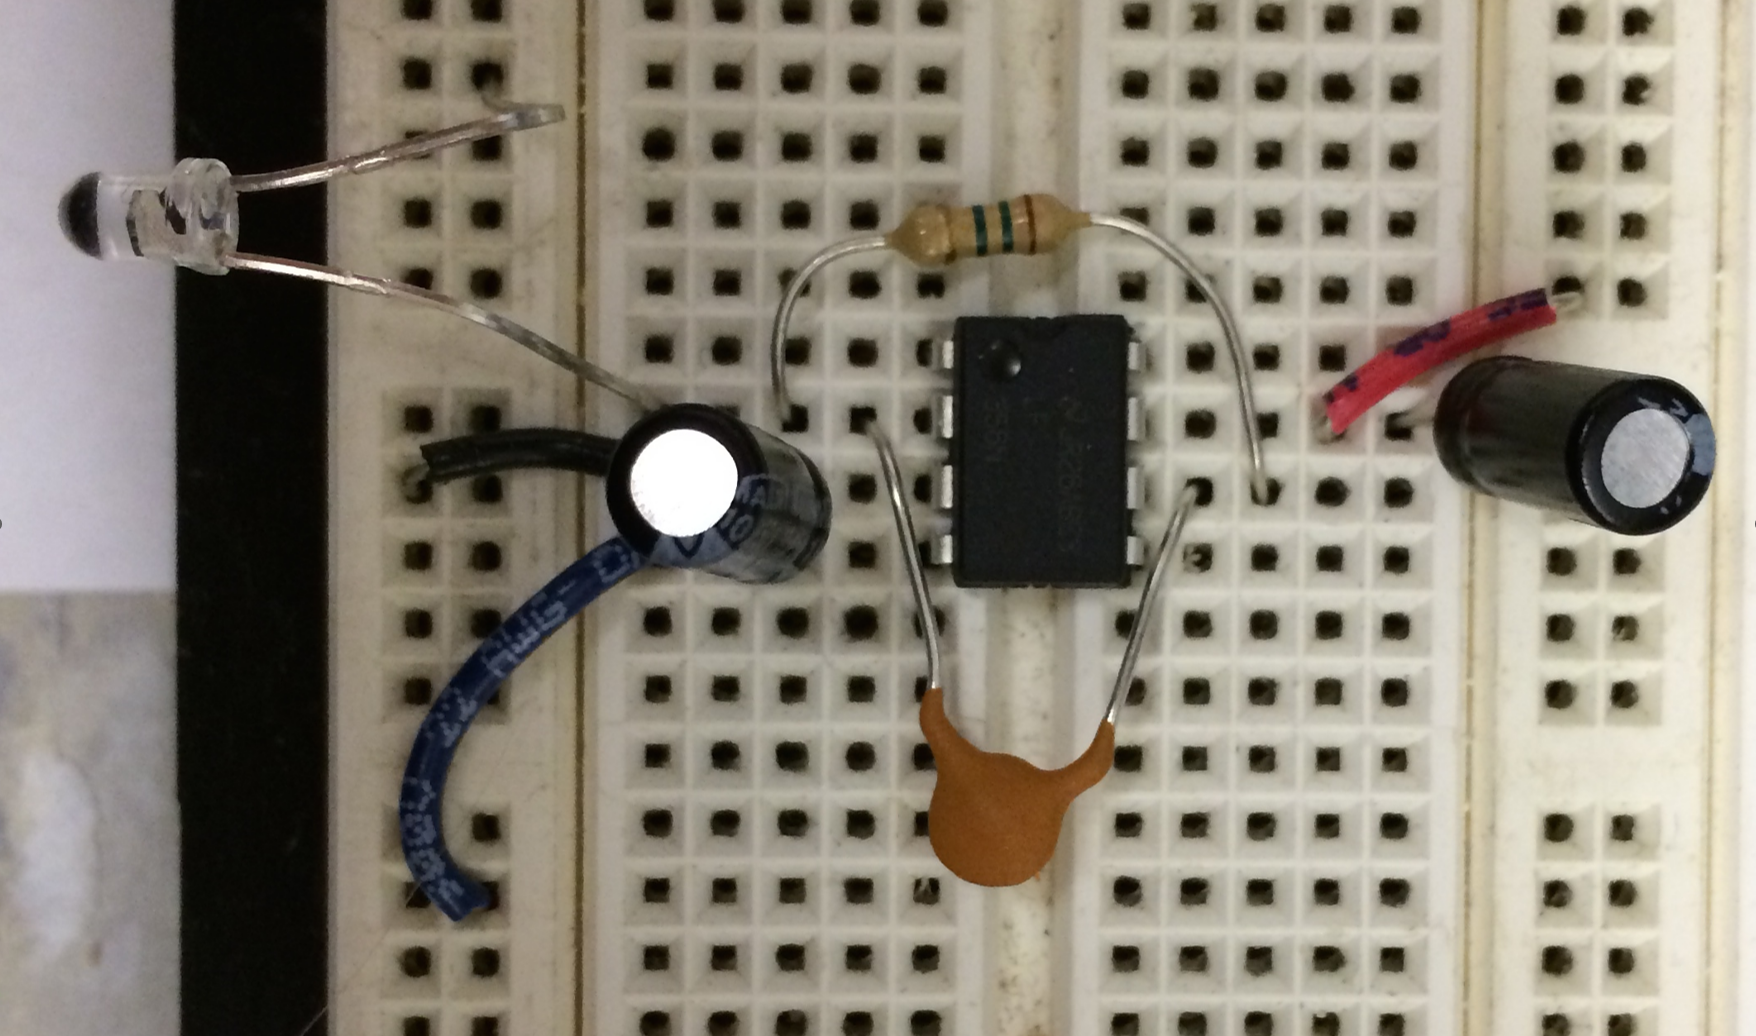
\includegraphics[width=10cm]{lab4fig/pb-example.png}
    \caption{Good placement of op-amp and bypass capacitors on a
protoboard. Note that short wires are used for all connections.}
    \label{pb}
\end{figure}

%------------------------------------------------

\section{General Op-Amp Tips}


\textbf{These are reminders of the basics steps you should always follow
when working with op-amps.}

\begin{enumerate}
\item
  This experiment will use both +15 V and --15 V to power the LF356
  op-amp. \textcolor{red}{Make sure you \textbf{unplug} the DC supplies while wiring
  your op-amp (you may find it useful to plug them into their own power
  strip). Everyone makes mistakes in wiring-up circuits. You should
  always check your circuit over before applying power.} Figure \ref{lf356} shows a
  pin-out for the LF356 chip. Familiarize yourself with the layout. The
  following procedure will help you wire up a circuit accurately:

  \begin{enumerate}
  \item
    Draw a complete schematic in your lab notebook, including all ground
    and power connections, and all IC pin numbers. Try to layout your
    prototype so the parts are arranged in the same way as on the
    schematic, as far as possible.
  \item
    Measure all resistor values before putting them in the circuit. Make
    sure you are using the correct capacitors. Some capacitors indicate
    the capacitance directly, but small capacitors usually just have a
    number where 10 = 10 pF, 102 = 10x10\textsuperscript{2} pF = 1 nF,
    103 = 10x10\textsuperscript{3} = 10 nF, 104 =
    10x10\textsuperscript{4} pF = 100 nF. Also, see the important note
    below about polarized capacitors.
  \item
    Adhere to a color code for wires. For example:

    \begin{itemize}
    \item
      \textcolor{OliveGreen}{0V (ground) Green}
    \item
      \textcolor{red}{+15V Red}
    \item
      \textcolor{blue}{-15V Blue}
    \end{itemize}
  \end{enumerate}
\item
  The op-amp chip sits across a groove in the prototyping board (see Figure \ref{pb}). Before inserting a chip, ensure the pins are straight (using a
  needle-nose pliers or something similar). After insertion, check
  visually that no pin is broken or bent under the chip. To remove the
  chip, use a small screwdriver in the groove to pry it out.
\item
  You will have less trouble with spontaneous oscillations if the
  circuit layout is neat and compact, in particular the feedback path
  should be as short as possible to reduce unwanted capacitive coupling
  (see Figure \ref{pb}). Also, wire around the chip rather than over it.
\item
  To help prevent spontaneous oscillations due to unintended coupling
  via the power supplies, use bypass capacitors to filter the power
  supply lines. A bypass capacitor between each power supply lead and
  ground will provide a miniature current ``reservoir'' that can quickly
  supply current when needed. This capacitor is normally in the range
  1--10 µF. \textcolor{red}{Compact capacitors in this range are usually
  \emph{\textbf{polarized}}, meaning that one terminal must always be
  positive relative to the other. If you put a polarized capacitor in
  backwards, it will burn out.} You will probably hear a pop and smell
  something foul. Please don't do this. The negative side should have an
  arrow on the capacitor. Also, the positive side should have a longer
  lead but this is not a good identification method as the leads can
  (and should) be cut. Bypass capacitors should be placed close to the
  op-amp pins. If you are connecting the +15 V supply to ground, the
  negative capacitor lead is connected to ground and the positive lead
  is connected to +15 V. If you are connecting the --15 V supply to
  ground, the negative capacitor lead is connected to --15 V and the
  positive lead is connected to ground.
\end{enumerate}
%------------------------------------------------

\section{Inverting Amplifier Application - Frequency Dependent Gain}


\begin{enumerate}
\def\labelenumi{\arabic{enumi}.}
\item
  Build the inverting amplifier shown in Figure \ref{invamp}, with \(R_F = 100 ~k\Omega\)
  and \(R = 10 ~k\Omega\). Measure \(R\) and \(R_F\) with the DMM before
  inserting them into the circuit board. Predict \(G_0\) and \(f_B\)
  from these measured values and the op-amp\textquotesingle s value of
  \(f_T\) from the data sheet. (You should be able to review your
  prelab work here!)
\item
  Use the function generator to measure the low frequency gain. What
  frequency should you use to test the low frequency gain (i.e., what
  frequency should the signal be below?) Consider the gain-bandwidth
  product and how it relates to your circuit. What is the predicted gain
  for the frequency you chose? Measure the low frequency gain \(G_0\) by
  measuring \(V_{in}\) and \(V_{out}\) using the scope (as you did in
  Lab 4). Do your measurements agree with your predictions?
\item
  Predict the 3 dB frequency for your circuit. Include your calculations
  in your lab book. Now, determine the 3 dB frequency experimentally.
  Describe the procedure you followed to determine \(f_B\). Does your
  measurement agree with your prediction? Explicitly record what
  criteria you used to determine whether or not the model and
  measurements agree.
\item
  Using the gain-bandwidth relation and your measurements of \(G_0\) and
  \(f_B\) to determine \(f_T\) for your op-amp. Does your measured value
  of \(f_T\) agree with the one from the datasheet?
\item
  Measure the frequency dependence of your circuit. Measure the gain at
  every decade in frequency from 10 Hz to 10 MHz. Should you use a 10X
  probe or coax cable to make your measurements? Explain your reasoning.
  Plot your measurements and predicted gain curve on the same plot.
  Where, if at all, is the simple model of the op-amp circuit not valid?
  Can you suggest possible model refinements and/or physical system
  refinements to get better agreement between the model predictions and
  measurements.
\end{enumerate}

%------------------------------------------------

\section{Summing Amplifier Application}

\subsection{First tests}


\begin{enumerate}
\def\labelenumi{\arabic{enumi}.}
\item
  Modify your basic inverting op-amp circuit to make it a summing
  amplifier as shown in Figure \ref{sumamp}. Use the component values you determined
  in your prelab for the resistors (you may want to check with your
  instructor to be sure they make sense). Draw the schematic in your
  notebook and label all components. Measure the resistors before
  inserting them into your circuit and record the values.
\item
  Determine the transfer function for your exact component values. What
  is \(V_{out}\) in terms of \(V_1\), \(V_2\), and \(V_3\)?
\item
  Confirm your summing amplifier is working according to your model by
  measuring \(V_{out}\) for different input voltages. Predict the output
  voltage for your set of test input voltages and measure \(V_{out}\).
  What is the best available measurement device to make these
  measurements? Why did you choose that device? Do your measurements
  agree with your predictions?
\end{enumerate}

\subsection{Digital-to-analog conversion}



Use your summing amplifier in ``digital to analog conversion mode'' to
create integer output voltages from 0 to --7 V from two input voltages
(0 V and 1 V). Predict what set of input voltages is required to get
each desired output voltage (\emph{Hint: You did this in your prelab}). Do your measurements agree with your predictions for all eight
voltages? How accurately were you able to make integer values of
voltage? Describe a way to refine the physical system to more accurately
create exact integer voltages.


%------------------------------------------------

\section{Integrator Application}


By now, you should be somewhat comfortable with experimental design and
reporting of outcomes, especially with op-amps and voltage dividers. In
this last section, you will design and characterize an integrator. Your
starting point should be the integrator circuit you designed in the
prelab. Items you likely wish to include in your lab notebook:

\begin{itemize}
\item
  Describe the circuit you are building and testing. It is suggested
  that you use R = 10 k$\Omega$ and the necessary capacitor to obtain a time
  constant of 1 ms.
\item
  Draw the schematic of the circuit with component values labeled.
\item
  List your predictions / models. It is fine to start by using ideal
  models.
\item
  How do you plan to test it? Be sure to use square, triangle, and sine
  waves at various frequencies.
\item
  The results of the tests with various inputs.
\item
  Do the results match your model? What didn't match?
\item
  How would you refine your model or physical system to get better
  agreement?
\end{itemize}

If you have an issue where the output seems to be at the rail voltage of
the op-amp, you likely have a DC signal on the input (in addition to the
AC signal). You should review the integrator theory section for ways to
alleviate this.
%------------------------------------------------

\section{Summary and Conclusions}

Write a two-paragraph summary in your lab notebook of what you learned
and any important takeaways.

%------------------------------------------------

\end{document}